\begin{figure}[!h]
  \centerline{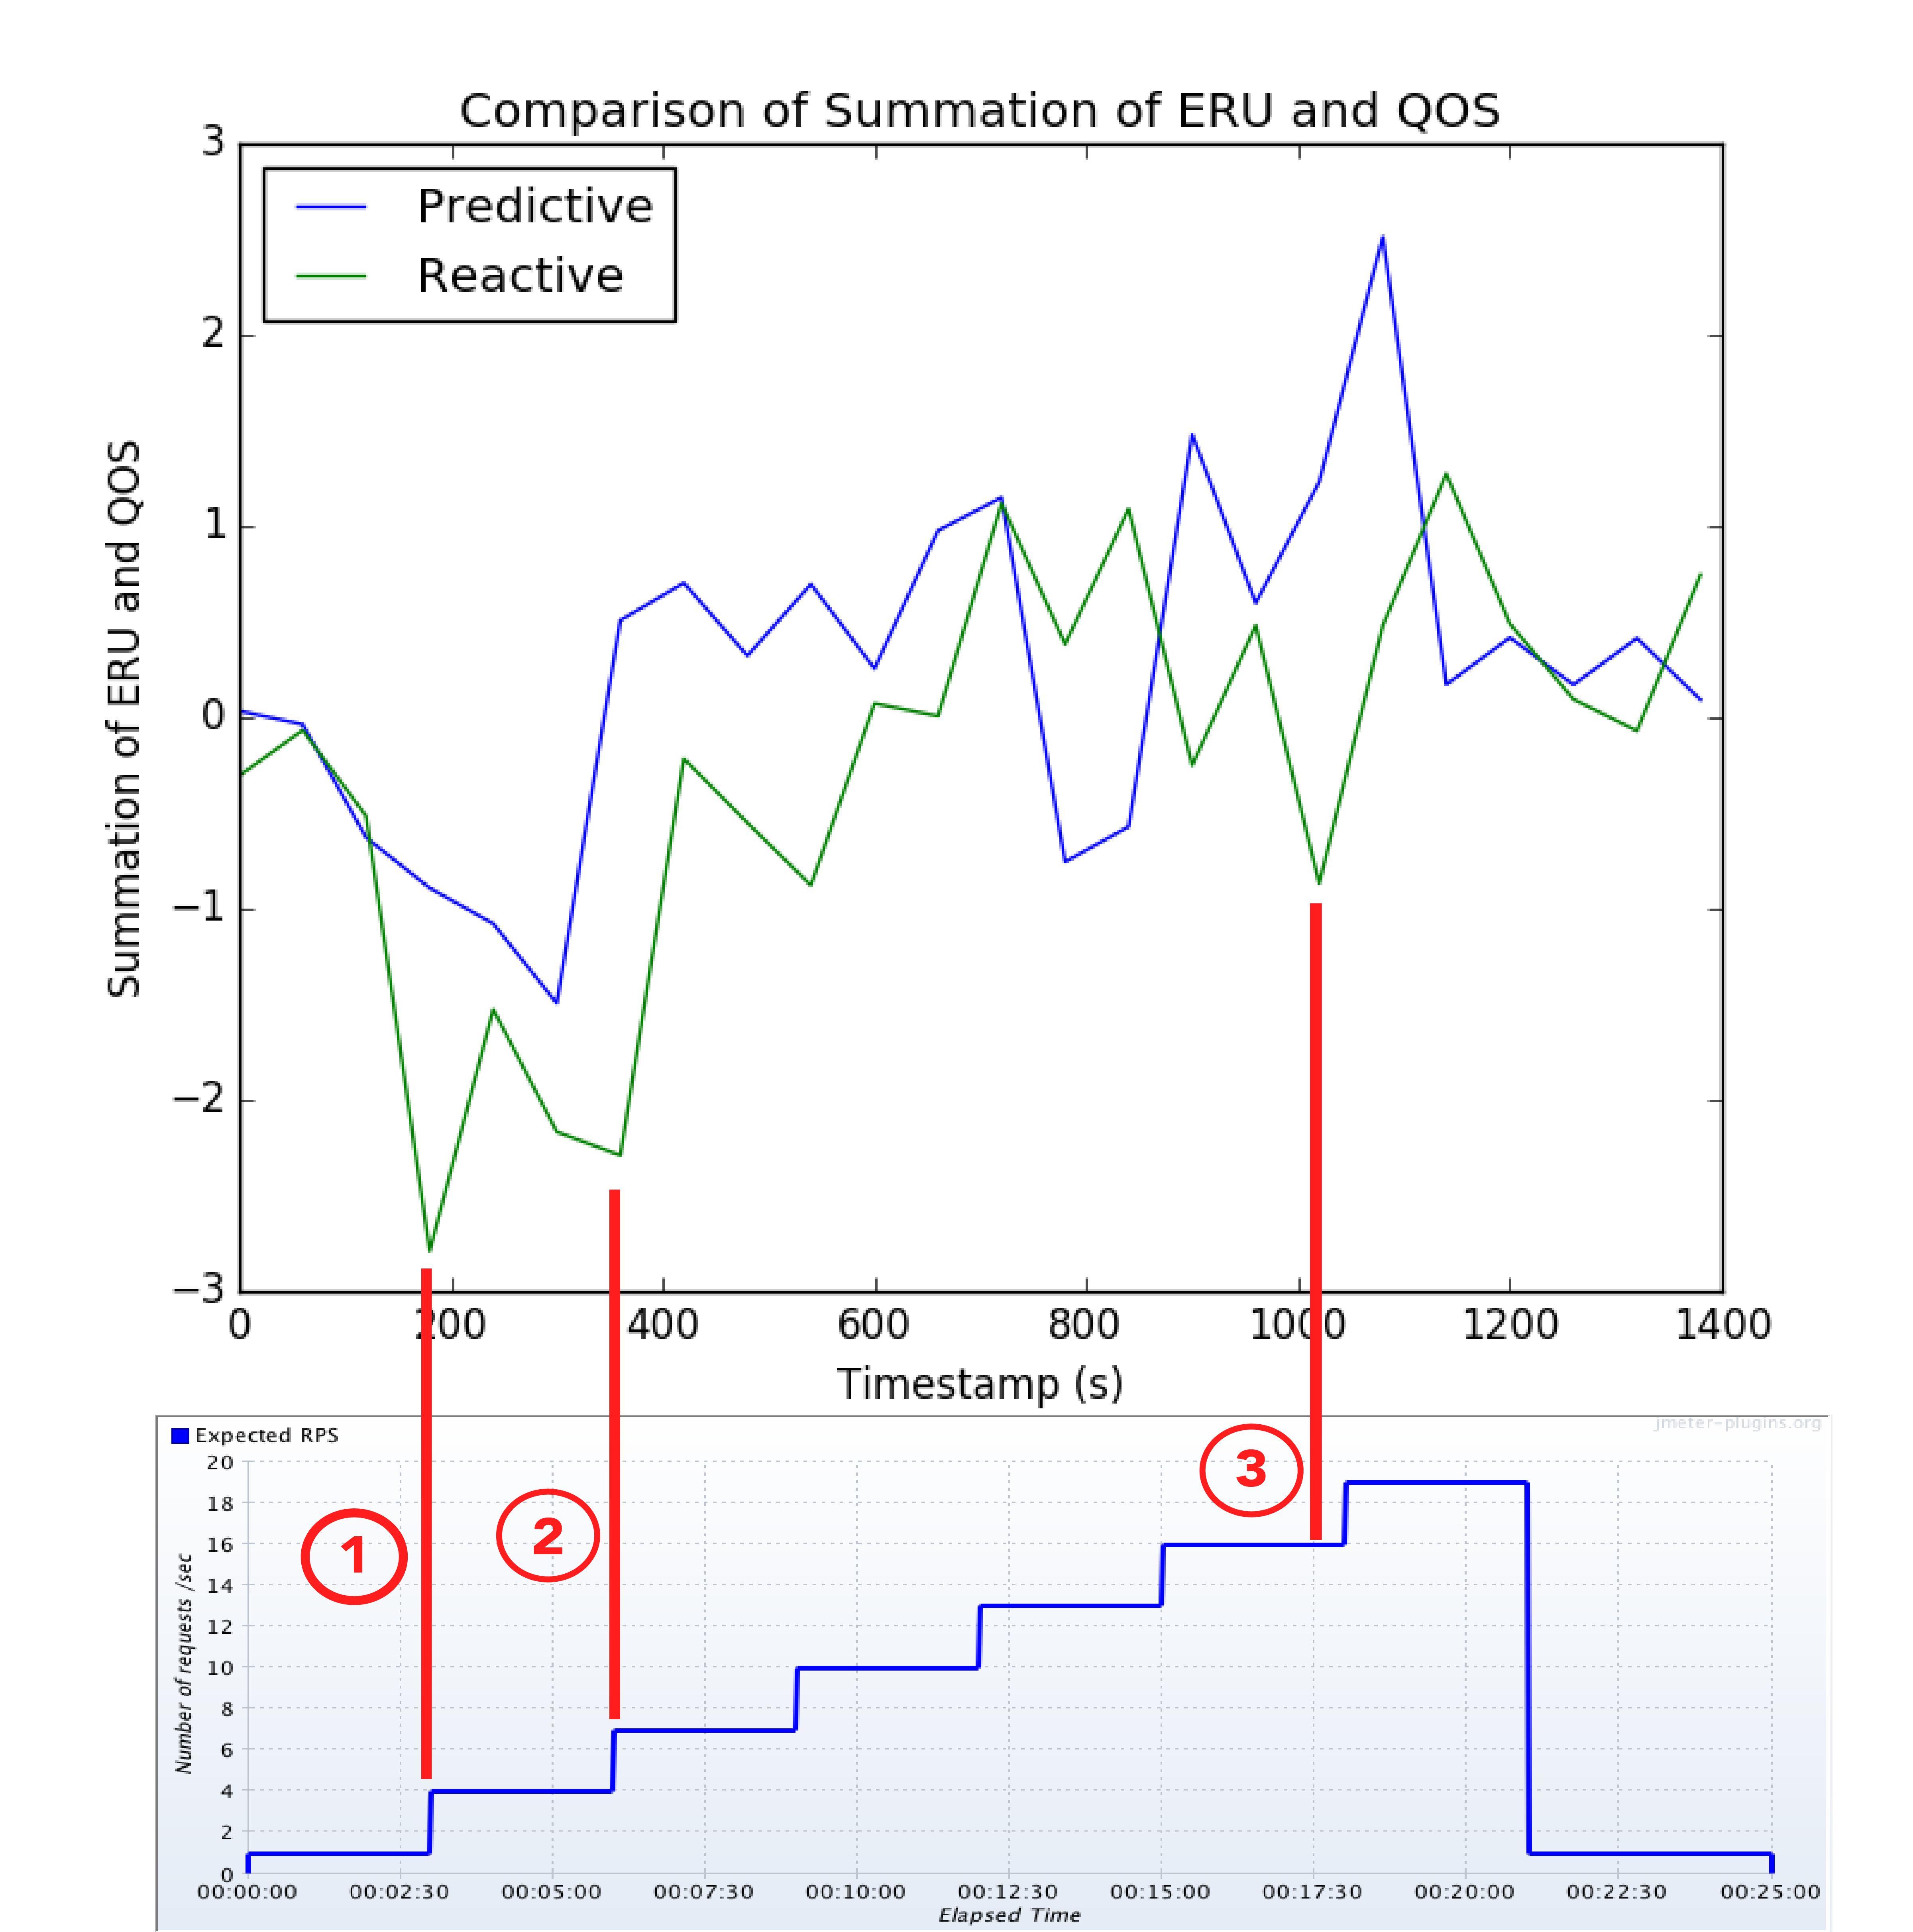
\includegraphics[scale=.70]{step-ladder-labelled.png}}
  \caption{A comparison of the summation of ERU and QoS for
    predictive and reactive auto-scaling for 135s, step-ladder}
  \label{fig:135s-step-ladder-labelled}
\end{figure}


Figure \ref{fig:135s-step-ladder-labelled} contains a graph
showing predictive and reactive auto-scaling's different
summations of efficient resource utilization and quality of service over the
course of trial. The traffic pattern super imposed below reflects the load
placed on the sample application, indicating the effect of the traffic pattern
on the summation of ERU and QoS. Given the larger the summation of ERU and QoS
the more desirable, times when the predictive line rises above the reactive line
reflect moments at which predictive auto-scaling is outperforming reactive
auto-scaling. Specifically, we can see three moments, labelled $1, 2,$ and
$3$ on the graph, in which predictive auto-scaling is particularly effective in
comparison to reactive auto-scaling. These moments help reveal a true strength of
predictive auto-scaling. While reactive auto-scaling under provisions because it
purely predicts based on the current moment, predictive auto-scaling is able to
recognize the general linearly upward pattern and auto-scale accordingly. As
such, the predictively auto-scaled application always has the resources it needs
to remain performant, as can be seen when examining the comparison of just
negated QoS in Figure \ref{fig:135s-step-ladder-only-qos}.\footnote{Again,
because we negated QoS when showing this graph, the larger the negated QoS
measure, the more performant the application, so it is desirable for the
predictive line to rise above the reactive line.} Finally, there is no cost in
ERU for auto-scaling, as can be seen when we just compare ERU in Figure
\ref{fig:135s-step-ladder-only-qos}.\footnote{This observation holds true
throughout the majority of the thesis. When the summation of predictive and
reactive auto-scaling diverges, it is because in variation of QoS. ERU stays
relatively constant between the two, which is necessary because it shows QoS
improvements are not coming at the cost of decreased ERU.
Thus for the remainder of the traffic
patterns we show only the summation of ERU and QoS with the understanding that
predominately QoS is contributing.} Overall, the included graphs clearly
demonstrate the benefits of predictive auto-scaling for this traffic pattern.

\begin{figure}[!h]
  \centerline{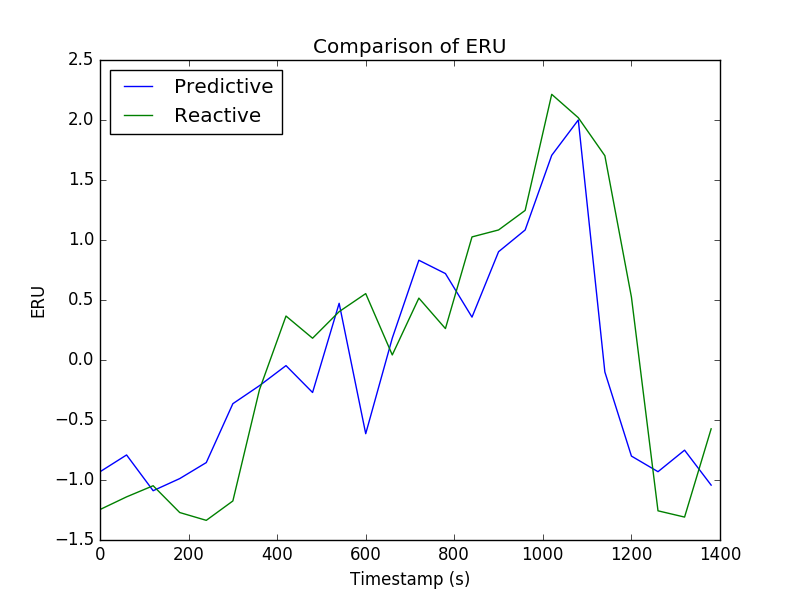
\includegraphics[scale=.70]{graph_135s_step-ladder_v2_only-eru.png}}
  \caption{A comparison of negated ERU for predictive and reactive auto-scaling
  for 135s, step-ladder}
  \label{fig:135s-step-ladder-only-eru}
\end{figure}

\begin{figure}[!h]
  \centerline{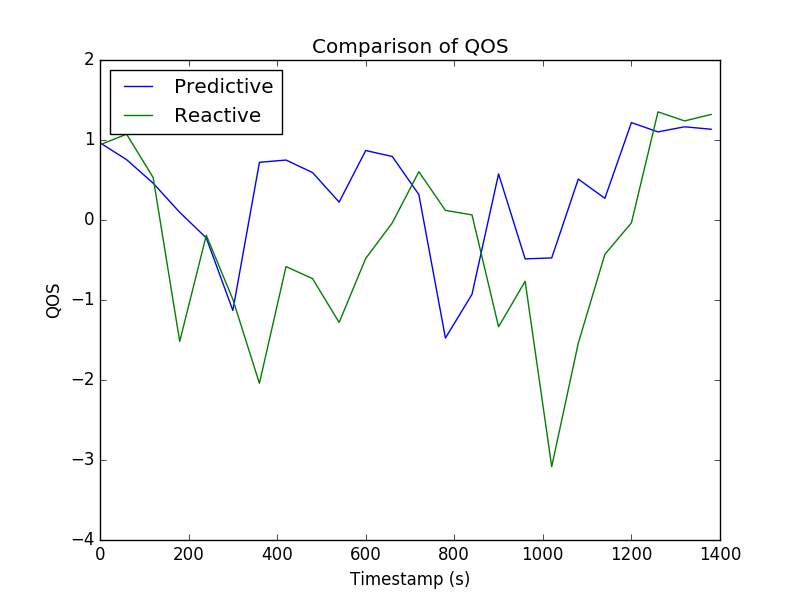
\includegraphics[scale=.70]{graph_135s_step-ladder_v2_only-qos.png}}
  \caption{A comparison of negated QoS for predictive and reactive auto-scaling
  for 135s, step-ladder}
  \label{fig:135s-step-ladder-only-qos}
\end{figure}

\begin{table}[htbp]
  \centering
  \caption{Difference in Predictive and Reactive Auto-scaling for 135s, step-ladder}
  \label{tab:135s-step-ladder}
\begin{tabular}{l c}\hline\hline
    \multicolumn{1}{c}{\textbf{Measure}} & \textbf{Value} \\ \hline
     p-value & 0.315 \\
     z-score & 0.482 \\
     std\_dev & 1.084 \\
     mean & 0.522
  \end{tabular}
\end{table}


While Figure \ref{fig:135s-step-ladder-labelled} shows the benefits of predictive
auto-scaling on the \textit{step-ladder} traffic pattern,
we are additionally interested in knowing if said benefits are
stastically significant.
As can be seen from the summary statistics in Table \ref{tab:135s-step-ladder},
with a p-value of .315 we are not
able to reject our null hypothesis that there is no difference between the
summation of ERU and QoS for predictive and reactive auto-scaling in favor of
our alternative hypothesis that there is a positive difference in the summation
of ERU and QoS for predictive and reactive auto-scaling. Essentially, this
p-value indicates that if there was truly no different between predictive and
reactive auto-scaling, we could expect to get these results about three out of
ten times we ran trials. Additionally, for the remainder of our trials with
different traffic patterns we were unable to obtain statistical significance.
This lack of statistical significance is likely the result of too little data,
given that we only ran one trial for each traffic-pattern, instead of combining
the results of multiple trials. Additionally, it may also be the case that the
inclusion of buffer periods, and periods when the requests per second are
sufficiently low such that only one pod needs to exist, is muting the
differences that occur when auto-scaling begins.
